\chapter[前言]{摘要} 
\label{cha:front}
\addcontentsline{toc}{section}{摘要}

在开放便捷的互联网环境下,能够进行实时有效的视频通讯,无疑是一个有充足重要性的议题。
我们以此为切入点,以实时、便捷、高效为目标,而进行项目设计。
 
在这样的实现设计下,我们甚至可以远程的动态的观测校园内实时情景。
\begin{figure}[h]
        \centering
                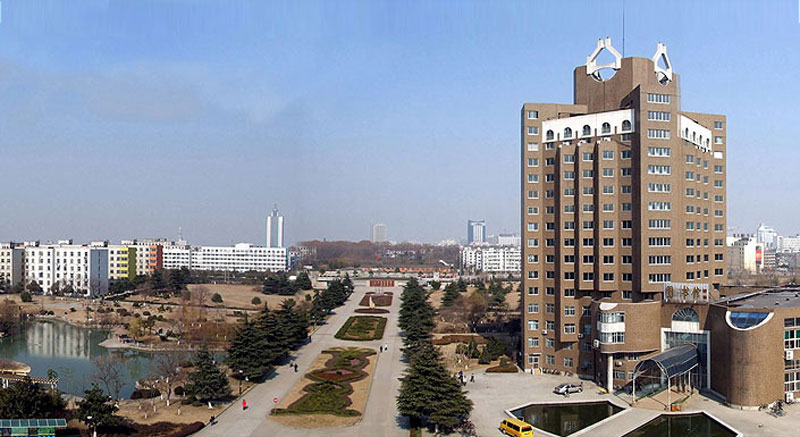
\includegraphics[width=.70\textwidth]{Figures/ch1.school.jpg}
        \caption{校园景观}
        \label{fig:executive}
\end{figure}

就这个需求来讲,某个特定的场所可能有诸多的信息需要开放介绍,甚至需要对
来访人员进行一定的导航、指引,而通过单一的静态信息可能无法达到较好的传
递效果,以此为出发点,我们力图构建一个系统来改善诸如此类的信息展示功能。

\begin{figure}[h]
        \centering
                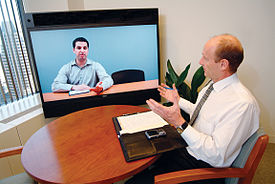
\includegraphics[width=.50\textwidth]{Figures/ch1.tele.jpg}
        \caption{静态的远程呈现}
        \label{fig:execimage2}
\end{figure}

对于这种有效信息的获取,其渠道是多元化的,在远程呈现的应用可能下,我们
可以将其作为一种获取方式进行设计。让身处远方的“参观者”能够“身临其境”的
感受环境,也即通过实时远程传递音频、视频等信息,并且让使用者“自主”的去
寻找他们感兴趣的信息。同时,这种功能不只是单向的,通过远程呈现的平台,
可以实现两地的人员的实时交流、咨询,也即实现一定的“虚拟出席”的功能,用
以辅助环境信息获取的效率。

一个可以令人感兴趣的设计是一种集散控制的导航、参观系统。

旨在某一建筑物中配置一套机群,其移动终端为可移动的并且具有网络传输功能
的“远程呈现机器人”,其基本功能是代替参观者虚拟出席到特定环境中,并获取
基本的环境信息,对于移动性的控制,一方面可以由非现场的参观者通过某一指
标(比如一张平面图的点击)来安全的(操作上存在一定的必要限制)控制移动,
另一方面可以由现场人员在移动终端上直接输入指令进行辅助控制,该辅助控制
也可以通过前述的平面图点击来封装化的实现。

这一套分布式地远程命令发送与获取,是通过一台服务器的命令转发来实现的,
用户通过网络与服务器建立连接,发送给定的指令,服务器负责将指令集中,再
转发到分散的特定的远程呈现机器人终端,这便是集散式系统的设计。
